\documentclass[11pt]{article}
\usepackage[margin=1in]{geometry}
\usepackage[utf8]{inputenc}
\usepackage[T1]{fontenc}
\usepackage{lmodern}
\usepackage{amsmath,amssymb}
\usepackage{graphicx}
\usepackage{booktabs}
\usepackage{xcolor}
\usepackage[hidelinks]{hyperref}
\usepackage{url}
\usepackage{caption}
\captionsetup{font=small,labelfont=bf}

\newcommand{\memprint}{MemPrint}
\newcommand{\secref}[1]{Section~\ref{#1}}
\newcommand{\figref}[1]{Figure~\ref{#1}}
\newcommand{\tabref}[1]{Table~\ref{#1}}
\newcommand{\term}[1]{\emph{#1}}

\title{What Is an Exact Memory Footprint Worth to a Scheduler?\\
Measured Footprints and Job Scheduling on Disaggregated Memory}
\author{Nafis Mustakin\\University of California, Riverside}
\date{October 2026}

\begin{document}
\maketitle

\begin{abstract}
A scheduler for a cluster with disaggregated memory can pack jobs only as tightly as its knowledge of each
job's memory footprint allows. We measure that knowledge for 25 programs at three inputs each, two LLM inference
engines among them, with the full Pin
trace as the truth, \memprint{}'s windowed and source-only estimates, Massif, DHAT, heaptrack, the gperftools heap
profiler and sampled RSS, and we replay the measured footprints through DMSched-Sim, a simulator of 32 nodes with
local DRAM and a shared 1\,TB pool, in which only the footprint oracle changes. Knowing a job's footprint curve
rather than its peak is where most of the gain lies: at 80\% offered load the exact curve gives a mean response
time 26.4$\times$ shorter than the user's request and 5.3$\times$ shorter than the exact peak, and it needs 5.0\,TB
of memory for a service level that the exact peak meets with 6.0\,TB and the request with 11.0\,TB. Among measured
estimators, \memprint{} windowed at 5\% is the only one that beats the exact peak (389 against 448 minutes), at
11 times the native run time against 227 times for the full trace. The heap profilers report the right peak for
most programs but read GCC's cc1 at 0.14 to 0.16 times its peak, llama2.c, whose weights are mapped from a file,
at 0.17 times and darknet at 1.97 times, so no margin makes them safe without over-reserving every other job; with
the LLM engines in the corpus, the calibrated margins of heaptrack and gperftools exceed twice their estimates. On a
stream of LLM jobs alone, only an earlier run's RSS peak, reactive resizing and exact knowledge avoid repeated OOM
kills, because the weights are touched within the first percent of a run, before \memprint{}'s first window and
outside every heap profiler's view. Curves built from DHAT's three recorded points
do worse than DHAT's peak under every margin. When the truth is the resident set on wall-clock time, every
measured curve, \memprint{}'s included, needs about 60\% headroom because its clock is not wall-clock time, and
peaks do better than curves, which shows that a footprint curve is useful to a scheduler only with a faithful
time axis.
\end{abstract}

\section{Introduction}
\label{sec:intro}

A batch scheduler places a job only after it decides how much memory to reserve for it, and on a cluster
with disaggregated memory that decision also sets how much of the shared pool the job takes away from other
jobs. Disaggregated memory attaches a pool of memory, over CXL or RDMA, that every node can use in addition to
its local DRAM~\cite{Li2023Pond,Zacarias2021Throughput}. The pool lets a cluster provision less local memory per
node, but only if the scheduler can pack jobs tightly, and it can pack them only as tightly as its knowledge
of each job's memory allows. Today that knowledge is weak. Peng et al.\ found that over 90\% of LLNL jobs use
under 15\% of a node's memory~\cite{Peng2020Underutilization}, and Zacarias et al.\ showed that a uniform 60\%
overestimate of memory demand cuts the throughput of a disaggregated system by about 25\% and raises the mean
response time about five times~\cite{Zacarias2021Accurate}.

Two kinds of knowledge are possible. A \term{peak} is one number per job, held for the whole run. A
\term{footprint curve} gives the memory the job needs at every point of its run, so a scheduler can let two
jobs whose peaks do not overlap share the same memory. The usual sources of either are the user's request,
a heap profiler such as Massif~\cite{ValgrindMassif}, DHAT~\cite{ValgrindDHAT}, heaptrack~\cite{heaptrack}
or the gperftools heap profiler~\cite{gperftools}, the resident set size (RSS) of an earlier run, a learned
predictor~\cite{Li2023Pond}, or a monitor that resizes a job's allocation while it
runs~\cite{Zacarias2023Dynamic}. \memprint{}~\cite{memprint} adds two more: a footprint curve measured by
instrumenting a sample of a run's memory accesses with Pin~\cite{Luk2005Pin}, and a footprint predicted from
the program's source code before it runs.

However, the simulators that study scheduling on disaggregated memory either model one run in cycle
detail with no scheduler~\cite{Puri2024DRackSim,CXLClusterSim,CXLDMSim,Yang2023CXLMemSim}, or treat a job's
memory as one declared peak with a synthetic error~\cite{Zacarias2021Accurate,Zacarias2021Throughput}. None
feeds the scheduler the footprints that real profilers report, and none compares those with a footprint
curve known before the job starts. It is therefore unclear how much better a scheduler does with an exact
footprint than with the tools that exist, and which property of the footprint (its peak, its shape over
time, or how safely it bounds the truth) the gain comes from.

In this work, we measure every source of footprint knowledge listed above on the same 25 programs and
replay the results through one scheduler, with everything but the footprint oracle held fixed. We make the
following contributions:
\begin{itemize}
  \item We build a corpus of footprint curves for 25 programs at three inputs each, HPC kernels, interpreters, a
    compiler and two LLM inference engines among them, from the full Pin trace
    (the truth), \memprint{}'s windowed and static estimates, Massif, DHAT, heaptrack, gperftools and sampled
    RSS, together with what each method costs (\secref{sec:corpus}).
  \item We build DMSched-Sim, a cluster simulator with local memory and a shared pool, an EASY-backfilling
    scheduler that admits a job only if its whole reservation curve fits, a remote-memory slowdown model and
    OOM kills (\secref{sec:sim}).
  \item We show how much of the gain an exact footprint brings comes from knowing the curve rather than the
    peak, how close each measured estimator gets, how much memory each needs for the same service, and what
    each estimator's cost buys (\secref{sec:results}).
  \item We evaluate curves derived from DHAT, which records no time series, and show why its three recorded
    points do not substitute for a measured curve (\secref{sec:dhat}).
  \item We schedule a stream of LLM inference jobs alone, whose memory is mostly model weights mapped from a file,
    and show which estimators survive it (\secref{sec:llm}).
\end{itemize}

\section{Background and related work}
\label{sec:related}

\paragraph{Disaggregated memory simulators.} DRackSim~\cite{Puri2024DRackSim},
CXL-ClusterSim~\cite{CXLClusterSim}, CXL-DMSim~\cite{CXLDMSim} and CXLMemSim~\cite{Yang2023CXLMemSim} model
the timing of accesses to pooled memory for one run, in cycle detail or from a trace, and none of them has a
job scheduler. The BSC Slurm simulator extended by Zacarias et al.\ schedules real job traces on a
disaggregated system~\cite{Zacarias2021Throughput}, but it represents a job's memory as one peak, and its study
of accuracy multiplies that peak by a synthetic overestimate~\cite{Zacarias2021Accurate}. Their dynamic
provisioning study resizes allocations from usage traces every five minutes~\cite{Zacarias2023Dynamic}, which
is a reactive monitor rather than knowledge available before the job starts. Boezennec et al.\ study the
allocation of disaggregated memory to jobs with piecewise-constant memory phases~\cite{Boezennec2024}, CFM
schedules jobs against per-job slowdown curves measured offline~\cite{Amaro2020CFM}, and Pond predicts the
untouched memory of virtual machines with a gradient-boosted model~\cite{Li2023Pond}. KS+ predicts the memory of
workflow tasks over time and reduces wasted GB-seconds by 51\% against peak-only prediction~\cite{KSplus2024},
but it has no cluster scheduler or memory pool.

\paragraph{Footprint estimators.} Massif samples the heap at up to 100 snapshots by default, on a time axis of
instructions or of milliseconds under Valgrind~\cite{ValgrindMassif}, and with \texttt{--pages-as-heap} it
counts mapped pages instead of heap blocks. DHAT reports the heap at its global peak (t-gmax) and at exit, and
the time of the peak, but no time series~\cite{ValgrindDHAT}. heaptrack records every allocation and can
export a heap curve~\cite{heaptrack}, and the gperftools heap profiler writes a dump each time the heap grows
by a set amount~\cite{gperftools}. All four count requested heap bytes, so they miss memory a program maps
itself and count blocks that are allocated but never touched. \memprint{} counts the bytes a program actually
touches, from a sample of its memory accesses~\cite{memprint}. Its windowed mode watches accesses only in
short windows (1\% or 5\% of the run) and tracks allocations and page residency in between, and its static
mode predicts the footprint from the source code with an interpreter that counts the references a build of
the program makes.

\section{Simulator}
\label{sec:sim}

DMSched-Sim replays one stream of jobs once per footprint oracle, so that any difference between two runs
comes from what the scheduler knows about memory. It is a time-slotted simulator (one slot is one minute)
written in Python (\texttt{analysis/memprint/sched/}).

\paragraph{System model.} The cluster has 32 nodes, each with 32 cores and 128\,GB of local DRAM, and one
shared pool of 1\,TB (one sixth of all memory). A job runs on one node. Its memory is placed in the node's
free local memory first, and the rest goes to the pool.

\paragraph{Jobs.} A job has an arrival time, a core count, a base runtime (its runtime with all memory
local), a true footprint curve $a(p)$ over its progress $p \in [0, 1]$, and a reservation curve $r(p)$ set by
the oracle. Curves are defined over progress rather than time, so a job slowed by remote memory stretches its
curve in wall-clock time.

\paragraph{Scheduler.} The scheduler is first come, first served with EASY backfilling~\cite{Lifka1995EASY}
over a window of 32 queued jobs. Each node keeps a timeline of committed local memory and cores, and the pool
keeps one of committed memory. A job starts on a node only if, at every slot from now to its projected end,
the part of its reservation that does not fit in the node's free local memory fits in the free pool. With a
time-varying reservation, two jobs whose peaks do not overlap can therefore share the same memory. When the
head of the queue cannot start, the scheduler reserves its earliest feasible start, and a later job may start
early only if it fits beside that reservation. Among the nodes that fit, the scheduler picks the one with the
least pool use and then the least free local memory left over (best fit).

\paragraph{Remote-memory slowdown.} Following the linear models of CFM~\cite{Amaro2020CFM} and Boezennec et
al.~\cite{Boezennec2024}, a job's runtime is stretched by the share of its resident GB-minutes that lie above
its local reservation:
\begin{equation}
T = T_{\mathrm{base}}\,(1 + \beta f_{\mathrm{remote}}), \qquad
f_{\mathrm{remote}} = \frac{\sum_t \max\bigl(0,\, a(t) - \ell(t)\bigr)}{\sum_t a(t)},
\end{equation}
where $\ell(t)$ is the local part of the reservation and $\beta = 0.5$, so a job whose memory is entirely remote
runs 1.5 times as long. Because the runtime depends on the placement and the placement depends on the runtime,
the two are solved together by fixed-point iteration when the job is admitted. The scheduler ranks candidate
nodes on the job's base runtime and then solves the stretch on the best node, falling back to the next node if
the stretched job no longer fits.

\paragraph{OOM kills.} If the true footprint exceeds the reservation at any slot, the job is killed there, its
work is lost, and it is requeued at the head of the queue with its reservation multiplied by 1.5, as a batch
system that raises a job's memory limit after an out-of-memory failure would do. A reactive oracle
(\secref{sec:oracles}) is the exception: its growth past the reservation is granted from free local memory or
the pool while either has room, and the job is killed only when neither does.

\paragraph{Metrics.} We report the mean response time (completion minus arrival), the mean bounded slowdown
(response over $\max(T_{\mathrm{base}}, 10\,\mathrm{min})$), the number of OOM kills, and the reserved and the
actually resident memory as shares of all memory. To leave out the warm-up and the drain of a finite stream,
every metric is taken over the jobs that arrive between the 10th and the 90th percentile of arrival times,
and the memory shares are averaged over that period.

\paragraph{Validation of the simulator.} Ten unit tests (\texttt{tests/sched/test\_sim.py}) check that two jobs
with non-overlapping peaks share a node under their curves but run one after the other under their peaks, that
an under-reservation is killed where the footprint passes it and requeued, that backfilling never delays the
head of the queue, that a fully remote job runs $1 + \beta$ times as long, and that elastic growth is granted
only from free memory. On the synthetic stream of the earlier prototype (3{,}000 jobs, five footprint shapes,
a 60\,GB median heap) the simulator reproduces the prototype's ordering at saturation: the exact curve sustains
101 jobs per hour, the exact peak 16\% fewer, a Massif-style curve 37\% fewer and a DHAT-style peak 57\% fewer.

\subsection{Job streams}
\label{sec:streams}

The main experiments use a controlled stream of 3{,}000 jobs in which memory is the contended resource. Each
job has 1 to 16 cores, a lognormal base runtime with a median of 30 minutes clipped to 5 to 720 minutes, and a
lognormal memory request with a median of 100\,GB. What a job really uses is its request multiplied by a ratio
$u \le 1$ taken from the LANL CM5 log of the Parallel Workloads Archive~\cite{PWA}, the archive log that records
both requested and used memory (median $u = 0.79$ over its 94{,}335 jobs with both fields). The shape of the job's
footprint, and what every estimator reports for it, come from one corpus program at its largest input
(\secref{sec:corpus}), chosen at random. All of that program's curves are scaled by the factor that puts the
truth's peak at the job's peak, so each estimator keeps its own over- or under-estimate. Arrivals are spread
evenly in random order over a span set so that the \term{offered load}, the resident GB-minutes arriving per
minute over the cluster's total memory, takes the values 0.4, 0.6, 0.8, 1.0 and 1.2. Each point is three
seeds.

We also tried the MetaCentrum2 log~\cite{PWA} (2013 to 2015, 5.7 million jobs with a memory request but no
used memory). In a window of 3{,}000 single-node jobs, 1\% of the jobs carry 92\% of the requested GB-minutes,
so the results of a replay depend on a handful of very large jobs. We therefore use the controlled stream for
the main results.

\subsection{Two truths}
\label{sec:truths}

\memprint{} counts the bytes a program touches, but a kernel charges and OOM-kills a process for its resident
pages. The two differ by page granularity, by memory an allocator keeps after a free, and by the runtime's own
pages (loader, libraries, MPI, an interpreter). We therefore run every experiment with two truths. With
\term{bytes touched} as the truth, the scheduler must cover the footprint a page-perfect system would need.
With \term{RSS} as the truth, it must cover the resident set sampled every 5\,ms. The runtime's own pages do
not grow with a job's data, so under the RSS truth only the RSS above the run's smallest sample (1.2 to 9.5\,MB
across the corpus) is scaled to the job's size.

\subsection{Oracles and margins}
\label{sec:oracles}

An oracle turns what is known about a job into its reservation curve. \tabref{tab:oracles} lists them. Curve
oracles follow a measured curve, coarsened to 20 windows over progress, each holding its largest value and
widened to its neighbours, because each method's clock (memory references for \memprint{}, instructions or
milliseconds under Valgrind for Massif, seconds for RSS) maps to wall-clock progress only approximately. Peak oracles hold one
value for the whole run.

\begin{table}[t]
\centering
\small
\caption{Footprint oracles. "Curve" oracles follow a measured footprint over the job's progress; "peak"
oracles hold one value for the whole run.}
\label{tab:oracles}
\begin{tabular}{lll}
\toprule
Oracle & Kind & Source \\
\midrule
Exact curve & curve & the truth, at full resolution (the upper bound) \\
Exact, 20 windows & curve & the truth, coarsened as the measured curves are \\
Exact peak & peak & the truth's peak \\
MemPrint windowed 1\%, 5\% & curve & \memprint{} watching 1\% or 5\% of the run \\
MemPrint pages only & curve & \memprint{} page residency, nothing watched \\
MemPrint static & curve & predicted from source before any run \\
Massif curve, pages-as-heap & curve & Massif snapshots (heap, or mapped pages), instruction clock \\
Massif, ms clock & curve & the same, with time in milliseconds under Valgrind \\
heaptrack curve & curve & heaptrack's heap over time \\
DHAT peak & peak & heap at DHAT's global peak (t-gmax) \\
DHAT curve, hold-then-decay & curve & three points recorded by DHAT (\secref{sec:dhat}) \\
gperftools peak & peak & largest in-use heap of the heap profiler's dumps \\
RSS peak & peak & peak RSS of an earlier run of the same input \\
User request & peak & the job's memory request \\
ML peak & peak & request $\times$ a 0.95-quantile gradient-boosted prediction of $u$ \\
Reactive resizing & curve & request for 5 minutes, then the last 5 minutes' largest use $+$ headroom \\
\bottomrule
\end{tabular}
\end{table}

The ML oracle follows Pond~\cite{Li2023Pond}. It predicts $u$ from the request, the core count, the requested
time and the user's and the executable's median $u$ in their history, with a gradient-boosted model at the
0.95 quantile, trained on half of the CM5 users. The jobs it predicts take their $u$ from the other half of the
users. The reactive oracle follows the dynamic provisioning of Zacarias et al.~\cite{Zacarias2023Dynamic}. The
scheduler is shown its future resizes when it admits the job, which favours this baseline.

Every estimate needs a margin, because an estimate below the truth causes OOM kills. A curve oracle's margin is
headroom added as a share of its own peak, since a curve on another clock can be low where the truth is not,
and no factor lifts a zero. A peak oracle's margin multiplies its peak. We use four margin policies: a fixed
10\% and 30\%, and two \term{calibrated} margins that a site could set from its own history. For each oracle and
program we compute the smallest margin with which the oracle never falls below the truth. A job then receives
the 90th percentile (\term{calibrated 90\%}) or the largest value (\term{calibrated 100\%}) of the other
programs' margins, so no oracle is tuned on the program it predicts. The request, ML and reactive oracles have no
profile to calibrate, and they keep a 10\% margin.


\section{Footprint corpus}
\label{sec:corpus}

We ran 25 programs at three inputs each, from the smallest to the largest, on a 32-core node with 62\,GB of
memory (\tabref{tab:corpus}): four PolyBench kernels~\cite{polybench} (2mm, gemm, jacobi-2d, atax, unoptimised
builds at SMALL, MEDIUM and LARGE), miniVite~\cite{minivite} with four threads, the GAP benchmarks bfs, pr, cc
and sssp on Kronecker graphs of $2^{16}$ to $2^{18}$ vertices, Lua, Python, Perl and SQLite workloads at three
sizes, GCC's cc1 compiling three source files at \texttt{-O0}, HPCCG, LULESH, NPB IS, CG and MG (classes S, W
and A), MiniFE, Quicksilver, Kripke, darknet classifying images with AlexNet (one input), and two LLM inference
engines: llama2.c~\cite{llama2c} generating 128 tokens from "Once upon a time" with the stories15M, 42M and 110M
models, and llama.cpp~\cite{llamacpp} (b11500, CPU, four threads) completing the same prompt with SmolLM2-135M
(32 and 128 tokens) and SmolLM2-360M (64 tokens), quantised to 8 bits, at the model's default 8192-token
context. Both engines map their weights from the model file rather than allocating them, and llama.cpp sizes its
KV cache for the whole context and clears it with \texttt{memset}. The native runs take 0.12 to 14.9\,s, and the
true peaks at the largest inputs are 15 to 450\,MB.

Every (program, input) ran under ten methods: the program alone, with its RSS sampled every 5\,ms; the full Pin
trace (\memprint{}'s splitter with frees tracked), which gives the bytes touched over time and is the truth;
\memprint{} windowed at 1\% and 5\% watched and pages only, with the tool built from the
\texttt{windowed-next} branch; Massif and Massif with \texttt{--pages-as-heap} (Valgrind 3.22, up to 1{,}000
snapshots), each run twice, with Massif's default clock of instructions executed and with milliseconds under
Valgrind; DHAT; heaptrack 1.3.0; and the gperftools 2.18 heap profiler with a
dump every 1/50 of the native peak RSS. The \memprint{} static predictions come from the C interpreter for
PolyBench (a curve over time) and from the C++ interpreter for HPCCG, LULESH and NPB (a whole-run footprint).
The NPB predictions are those of the second blind test, made before any trace of NPB existed; the static route
does not cover the LLM engines. Of the 874 runs, two failed: the full traces of NPB MG class A and of llama.cpp with
the 360M model ran out of memory (the latter at 20.7\,GB, in Pin's allocator), so MG is used up to class W and
llama.cpp up to the 135M model with 128 tokens. The runs shared the node with up to 15 others (the LLM runs with
up to 7), so the costs below are slowdowns under load.

\begin{table}[t]
\centering
\caption{The corpus at each program's largest input: the true peak (bytes touched), the mean over the run as a
share of the peak, each method's peak as a share of the true peak, and the time each method takes over the
native run.}
\label{tab:corpus}
\resizebox{\textwidth}{!}{\begin{tabular}{llrrrrrrrrrrrr}
\toprule
 & & \multicolumn{7}{c}{Footprint (ratios to the true peak)} & & \multicolumn{4}{c}{Cost (time / native)} \\
\cmidrule(lr){3-9} \cmidrule(lr){11-14}
Program & Input & Peak (MB) & Mean/peak & RSS & MemPrint W5 & Massif & DHAT & heaptrack & Native (s) & W5 & Massif & DHAT & Full trace \\
\midrule
2mm & LARGE & 37.1 & 0.96 & 1.03 & 1.00 & 1.00 & 1.00 & 1.00 & 8.6 & 4.8 & 5.6 & 15.2 & 357 \\
atax & LARGE & 32.1 & 0.87 & 1.04 & 1.00 & 1.00 & 1.00 & 1.00 & 0.1 & 21.8 & 5.7 & 9.8 & 122 \\
GCC cc1 & large & 105.5 & 0.69 & 1.27 & 1.06 & 0.16 & 0.15 & 0.15 & 1.8 & 100.5 & 11.0 & 68.1 & 206 \\
darknet & alexnet & 269.9 & 0.86 & 1.07 & 1.04 & 1.97 & 1.97 & 1.97 & 3.0 & 11.8 & 10.5 & 45.9 & 773 \\
GAP bfs & 18 & 72.8 & 0.36 & 1.05 & 1.00 & 0.99 & 0.99 & 0.99 & 1.5 & 8.1 & 3.0 & 5.7 & 83 \\
GAP cc & 18 & 72.0 & 0.36 & 1.06 & 1.01 & 1.01 & 1.01 & 1.01 & 2.2 & 5.5 & 2.2 & 3.9 & 56 \\
GAP pr & 18 & 72.4 & 0.40 & 1.05 & 1.01 & 1.00 & 1.00 & 1.00 & 2.8 & 5.2 & 2.3 & 5.3 & 123 \\
GAP sssp & 18 & 135.8 & 0.36 & 0.95 & 1.00 & 1.00 & 1.00 & 1.00 & 2.5 & 5.9 & 2.4 & 4.4 & 116 \\
gemm & LARGE & 29.1 & 1.00 & 1.04 & 1.00 & 1.00 & 1.00 & 1.00 & 6.1 & 4.4 & 5.7 & 15.2 & 356 \\
HPCCG & 64 & 102.7 & 0.99 & 1.03 & 1.00 & 1.02 & 1.02 & 1.02 & 1.7 & 13.3 & 10.5 & 24.8 & 310 \\
jacobi-2d & LARGE & 27.1 & 1.00 & 1.04 & 1.00 & 1.00 & 1.00 & 1.00 & 12.8 & 3.7 & 7.3 & 16.2 & 275 \\
Kripke & 16 & 274.6 & 0.88 & 1.02 & 1.00 & 1.00 & 1.00 & 1.00 & 3.4 & 11.4 & 4.8 & 50.7 & 473 \\
llama2.c & 110M & 449.7 & 0.98 & 1.14 & 1.00 & 0.17 & 0.17 & 0.17 & 14.9 & 3.5 & 3.6 & 20.5 & 41 \\
llama.cpp & 135m-n128 & 352.9 & 0.89 & 1.08 & 1.00 & 1.05 & 1.05 & 1.05 & 1.5 & 47.1 & 137.1 & 279.6 & 604 \\
Lua & 1 & 57.1 & 0.53 & 1.15 & 0.94 & 1.02 & 0.92 & 0.92 & 4.2 & 14.8 & 4.3 & 28.0 & 161 \\
LULESH & 60 & 151.1 & 0.62 & 1.02 & 1.00 & 1.00 & 1.00 & 1.00 & 5.5 & 10.6 & 7.9 & 32.2 & 458 \\
miniVite & 32768 & 15.4 & 0.51 & 1.99 & 1.00 & 1.55 & 1.53 & 1.42 & 1.8 & 42.5 & 22.9 & 36.9 & 322 \\
MiniFE & 80 & 256.5 & 0.98 & 1.04 & 1.00 & 1.03 & 1.02 & 1.02 & 9.2 & 10.7 & 6.7 & 23.8 & 273 \\
NPB CG & A & 27.4 & 1.00 & 1.10 & 1.00 & 0.99 & 0.99 & 0.99 & 1.9 & 10.6 & 7.8 & 15.5 & 237 \\
NPB IS & A & 69.7 & 0.81 & 1.03 & 1.00 & 0.99 & 0.99 & 0.99 & 2.4 & 3.9 & 2.7 & 7.0 & 61 \\
NPB MG & W & 58.5 & 0.98 & 1.04 & 1.00 & 0.99 & 0.99 & 0.99 & 0.5 & 15.5 & 4.0 & 8.8 & 107 \\
Perl & 1 & 56.1 & 0.67 & 1.15 & 0.97 & 1.04 & 0.97 & 0.96 & 1.8 & 30.9 & 5.2 & 44.8 & 145 \\
Python & 1 & 95.9 & 0.37 & 1.19 & 1.04 & 1.29 & 1.01 & 0.14 & 5.6 & 17.0 & 12.5 & 175.5 & 272 \\
Quicksilver & 100000 & 42.2 & 1.00 & 1.28 & 1.01 & 1.02 & 1.01 & 1.01 & 5.5 & 13.9 & 6.3 & 44.5 & 227 \\
SQLite & 1 & 77.8 & 0.43 & 1.06 & 0.97 & 1.01 & 1.01 & 1.01 & 1.2 & 47.7 & 7.1 & 39.0 & 204 \\
\bottomrule
\end{tabular}
}
\end{table}

\subsection{Accuracy of the peak}

\begin{figure}[t]
\centering
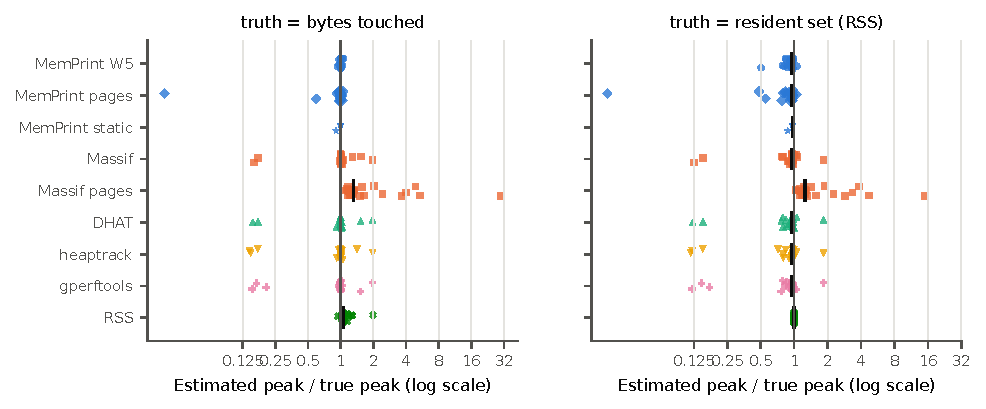
\includegraphics[width=\textwidth]{figures/peak_accuracy.pdf}
\caption{Each method's peak over the true peak, every program at its largest input (one marker per program,
the black bar is the median). Left: against bytes touched. Right: against the RSS.}
\label{fig:peak}
\end{figure}

Most heap profilers report the right peak for most of these programs, and fail badly on the rest
(\figref{fig:peak}). Specifically, Massif's peak is within 5\% of the true peak on 20 of the 25 programs, DHAT
and gperftools on 20 and heaptrack on 19, because these programs touch nearly all the heap they allocate.
However, the heap profilers read 0.14 to 0.16 times the peak of GCC's cc1, whose garbage collector maps its own
pages, and 0.17 times that of llama2.c, whose 110M model's weights are mapped from the file and never pass
through the heap; they read 1.97 times the peak of darknet and 1.42 to 1.55 times that of miniVite, which allocate
memory they never touch. On llama.cpp they are within 5\% (1.04 to 1.05), because its weights' file mapping is
offset by a KV cache that it allocates on the heap and clears in full. \memprint{} windowed at 5\% is within 5\%
on 23 of the 25 programs (0.94 to 1.06 times the truth). Pages only is within 5\% on 21; it estimates the
resident pages of heap blocks and writable sections, so it misses the read-only weight mappings and reads
llama2.c at 0.02 and llama.cpp at 0.60. Massif with \texttt{--pages-as-heap} overestimates every program (1.07 to
29.9 times), and the RSS is 0.95 to 1.99 times the bytes touched (median 1.05).

\subsection{Shape over time}

\begin{figure}[t]
\centering
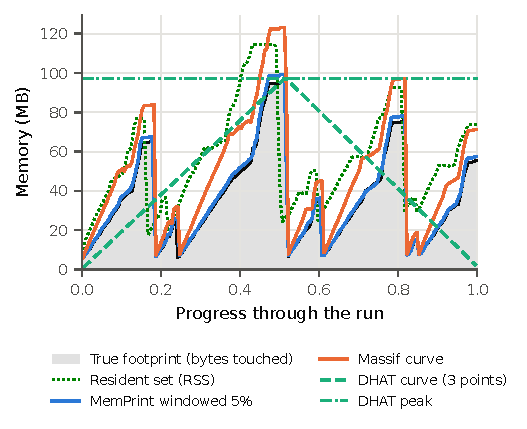
\includegraphics[width=0.6\textwidth]{figures/motivation_curve.pdf}
\caption{Python (largest input): the true footprint over the run, the RSS, and the curves and peaks the
estimators report. Each curve is on its own method's clock, rescaled to progress.}
\label{fig:motivation}
\end{figure}

The footprint of half of the programs varies over the run. The mean over the run is below 70\% of the peak for
11 of the 25 programs (GCC's cc1, the four GAP kernels, Lua, LULESH, miniVite, Perl, Python and SQLite), and it
is 0.36 to 0.40 times the peak for the four GAP kernels. A scheduler that holds the peak for such a job reserves memory that
the job leaves unused for most of its run. \figref{fig:motivation} shows Python's footprint, which rises and
falls seven times. \memprint{} windowed at 5\% follows it within a few percent. Massif's curve, on its clock of
instructions, follows its phases but sits above it, because Massif counts requested heap bytes and Python
allocates memory it never touches (1.29 times the true peak).
DHAT records only the peak, its time and the heap at exit, so a curve built from those points misses every phase
but one.

\begin{figure}[t]
\centering
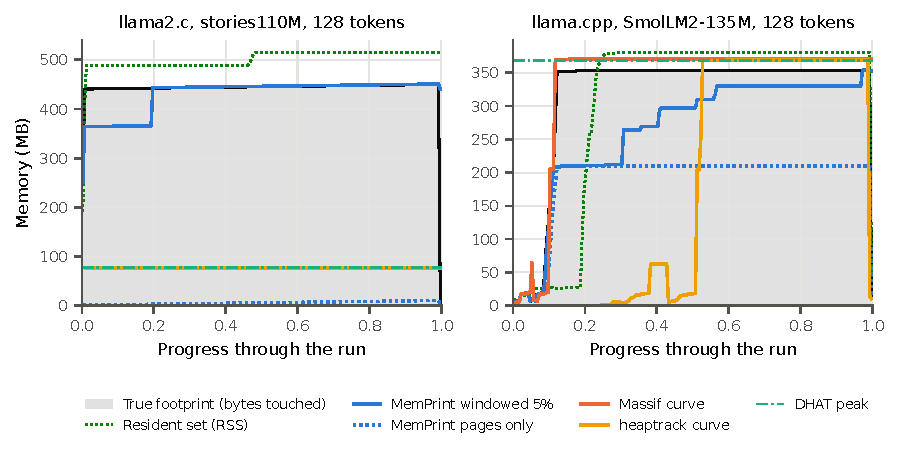
\includegraphics[width=\textwidth]{figures/llm_curves.pdf}
\caption{The two LLM engines at their largest inputs: the true footprint over the run, the RSS, and the curves
and peaks the estimators report, each on its own clock rescaled to progress.}
\label{fig:llmcurves}
\end{figure}

The LLM engines differ from the rest of the corpus in where their memory is (\figref{fig:llmcurves}). Both map
the model's weights from the file, and both read all of them for the first token, so the true footprint reaches 90\%
of its peak within the first 1 to 2\% of a llama2.c run and stays there (mean 0.96 to 0.98 of the peak). llama.cpp
reaches it at 12\% of a 128-token run, and its mean is 0.89 of the peak.
The heap profilers see only the heap: 0.08 to 0.21 of llama2.c's peak, and the KV cache and compute buffers of
llama.cpp. \memprint{} windowed at 5\% reaches about the right peak (0.86 to 1.00 over the five configurations), but late: its curve reaches 90\% of
the peak at 19 to 20\% of a llama2.c run and at 56\% of the llama.cpp run, because between its windows it tracks
heap blocks and writable pages, not a read-only file mapping, so it learns of the weights only when a window
watches the program reading them. Pages only, which never watches, reads llama2.c at 0.02 to 0.05 of its peak.

\subsection{Cost}

\begin{figure}[t]
\centering
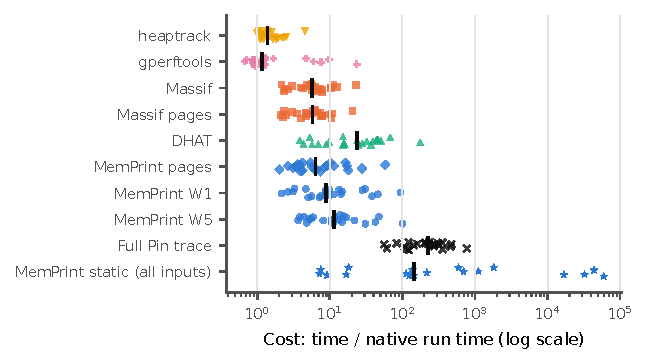
\includegraphics[width=0.6\textwidth]{figures/cost.pdf}
\caption{Each method's time over the native run, every program at its largest input (static: every input with a
prediction). The black bar is the median.}
\label{fig:cost}
\end{figure}

\memprint{}'s windowed estimates are not cheaper than the heap profilers on these short runs
(\figref{fig:cost}). At the largest inputs, the median slowdown is 1.4$\times$ for heaptrack, 1.2$\times$ for
gperftools, 5.7$\times$ for Massif (6.4$\times$ with its clock in milliseconds) and 23.8$\times$ for DHAT, against 6.3$\times$ for \memprint{} pages only,
8.9$\times$ at 1\% watched and 11.4$\times$ at 5\% watched. The full Pin trace costs 226.8$\times$ (41.2 to
772.5$\times$). The two LLM engines sit at the ends of that range. llama2.c, a single-threaded run of 2 to
15\,s, costs 41 to 49$\times$ under the full trace, 3.5 to
6.6$\times$ under \memprint{} at 5\% and 19 to 21$\times$ under DHAT. llama.cpp, a sub-second run with four
threads, costs 469 to 604$\times$ under the full trace, 47 to 91$\times$ under \memprint{} at 5\%, 82 to
137$\times$ under Massif and 182 to 280$\times$ under DHAT, while heaptrack and gperftools stay at 2.4 to
5.8$\times$. Pin's fixed start-up cost weighs heavily on runs of a few seconds, and the windowed mode is
slowest on programs with much code to re-translate (GCC's cc1, 93.6$\times$ at 1\%). The static route needs no
run of the program, but its interpreter takes 7 to 59{,}000 times the native run. It predicts atax MEDIUM in
0.8\,s, the other PolyBench kernels at MEDIUM in 13 to 24\,s and HPCCG in 255 to 989\,s, but NPB IS and CG at
class W take 4.0 and 5.5 hours.

\subsection{Static predictions}

The static predictions are within 0.46\% of the true peak at the median, over the 19 (program, input) pairs
they cover. They fail in two known ways. For LULESH, the static route predicts the footprint of the whole run,
1.57 times the live peak, because LULESH frees and reallocates its arrays between iterations and the static
route does not model frees for C++ programs. For NPB MG, the prediction is 7 to 9\% short, as it was in the
blind test, for a reason we have not found.


\section{Results}
\label{sec:results}

We first ask how much an exact footprint is worth and where the gain comes from, then how close each measured
estimator gets, and finally what each estimator's cost buys. \tabref{tab:load08} gives every oracle at offered
load 0.8 with calibrated 90\% margins, and \figref{fig:load} gives the response time across loads.

\begin{table}[t]
\centering
\caption{Every oracle at offered load 0.8, calibrated 90\% margins (10\% for the request, ML and reactive
oracles, which have no profile to calibrate), mean of three seeds. Resp.\ is the mean response time, BSLD the
mean bounded slowdown, Kills the OOM kills per stream of 3{,}000 jobs, Res.\ and Used the memory reserved and
actually resident as a share of all memory.}
\label{tab:load08}
\resizebox{\textwidth}{!}{\begin{tabular}{lrrrrrrrrrr}
\toprule
 & \multicolumn{5}{c}{Truth = bytes touched} & \multicolumn{5}{c}{Truth = RSS} \\
\cmidrule(lr){2-6} \cmidrule(lr){7-11}
Oracle & Resp. (min) & BSLD & Kills & Res. \% & Used \% & Resp. (min) & BSLD & Kills & Res. \% & Used \% \\
\midrule
Exact curve & 90 & 2.7 & 0 & 79 & 79 & 91 & 2.7 & 0 & 80 & 80 \\
Exact, 20 windows & 158 & 5.6 & 0 & 81 & 72 & 168 & 6.0 & 0 & 80 & 72 \\
MemPrint windowed 1\% & 358 & 14.2 & 375 & 81 & 63 & 1814 & 78.2 & 330 & 59 & 33 \\
MemPrint pages only & 381 & 15.3 & 377 & 79 & 63 & 1811 & 78.0 & 341 & 59 & 33 \\
MemPrint windowed 5\% & 391 & 15.7 & 391 & 77 & 61 & 1807 & 77.9 & 316 & 59 & 33 \\
Exact peak & 460 & 18.8 & 0 & 78 & 58 & 436 & 17.8 & 0 & 78 & 60 \\
Reactive resizing (5 min) & 589 & 24.6 & 20 & 71 & 54 & 630 & 26.4 & 20 & 70 & 54 \\
MemPrint windowed 5\%, peak & 832 & 34.9 & 391 & 73 & 48 & 1038 & 44.0 & 513 & 69 & 45 \\
RSS peak (earlier run) & 930 & 39.4 & 382 & 69 & 44 & 436 & 17.8 & 0 & 78 & 60 \\
gperftools peak & 955 & 40.3 & 1308 & 70 & 44 & 1281 & 54.6 & 1309 & 66 & 41 \\
DHAT peak & 979 & 41.4 & 912 & 70 & 45 & 1277 & 54.4 & 921 & 66 & 40 \\
heaptrack curve & 1077 & 45.6 & 1512 & 67 & 41 & 3075 & 133.3 & 1668 & 49 & 23 \\
ML peak (quantile GBM) & 2006 & 86.6 & 115 & 61 & 29 & 1971 & 85.2 & 115 & 61 & 30 \\
Massif curve & 2175 & 94.0 & 729 & 56 & 27 & 2408 & 104.0 & 1027 & 55 & 29 \\
User request & 2215 & 95.8 & 0 & 57 & 27 & 2197 & 95.1 & 0 & 57 & 28 \\
DHAT curve (3 points) & 3443 & 149.7 & 708 & 51 & 22 & 3074 & 133.5 & 806 & 51 & 24 \\
Massif curve, ms clock & 3973 & 173.5 & 1827 & 44 & 15 & 2554 & 110.4 & 1026 & 53 & 26 \\
DHAT hold-then-decay & 4342 & 188.7 & 708 & 48 & 20 & 3983 & 172.8 & 806 & 48 & 21 \\
Massif pages-as-heap & 4594 & 200.1 & 617 & 42 & 16 & 4452 & 193.7 & 643 & 41 & 16 \\
Massif pages-as-heap, ms clock & 6777 & 296.1 & 384 & 36 & 11 & 5889 & 256.8 & 759 & 38 & 12 \\
\bottomrule
\end{tabular}
}
\end{table}

\begin{figure}[t]
\centering
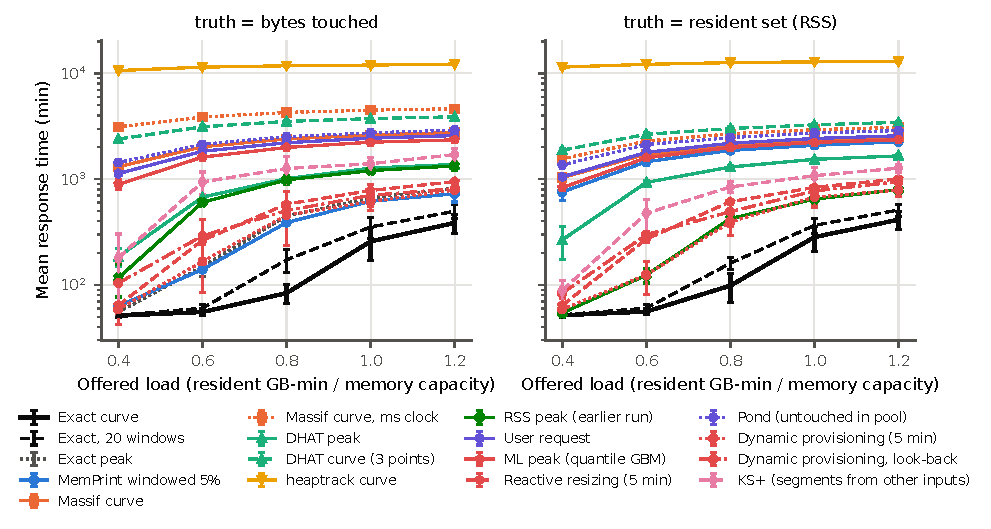
\includegraphics[width=\textwidth]{figures/response_vs_load.pdf}
\caption{Mean response time against offered load, calibrated 90\% margins (95\% confidence intervals over three
seeds, log scale). Left: the truth is bytes touched. Right: the truth is the RSS.}
\label{fig:load}
\end{figure}

\subsection{An exact footprint curve}

Knowing a job's footprint curve, rather than its peak, is where most of the gain lies. At load 0.8 the exact
curve gives a mean response time of 84 minutes, against 448 minutes for the exact peak and 2{,}208 minutes for
the user's request, under the bytes-touched truth, which makes the curve 26.4$\times$ better than the request and
5.3$\times$ better than the peak, and the peak 4.9$\times$ better than the request. The RSS truth gives the same
picture (99, 423 and 2{,}183 minutes). The curve lets the scheduler keep 81\% of all memory resident with jobs,
against 58\% for the exact peak and 27\% for the request, because jobs whose peaks fall at different times share
the memory that a peak would hold idle. Coarsening the exact curve to the 20 widened windows used for every
measured curve raises the response to 173 minutes, so about three quarters of the curve's advantage over the peak
survives the resolution and the timing slack a measured curve needs.
The gap widens with load (\figref{fig:load}). At load 0.4 every oracle that does not over-reserve keeps
up with arrivals, and from load 0.6 the peak and the request saturate memory while the curve does not.

\subsection{Measured estimators}

\memprint{} windowed at 5\% is the only measured estimate that beats the exact peak, and only under the
bytes-touched truth. With calibrated 90\% margins it gives 389 minutes, against 448 minutes for the exact peak,
469 for \memprint{} pages only, 580 for reactive resizing, 765 for \memprint{} windowed at 1\%, and 985 and 1{,}011
minutes for the RSS and DHAT peaks. The LLM engines cost the other two \memprint{} curves their place: without
them, pages only and windowed at 1\% gave 381 and 358 minutes, but their curves lag the weights the engines read
at the start (\secref{sec:corpus}), and the margin that covers 90\% of the programs rises from 4 to 8\% for pages
only and from 5 to 14\% for windowed at 1\% (\tabref{tab:margins}), with 1{,}117 to 1{,}901 OOM kills per stream.
The \memprint{} 5\% curve still loses to the exact curve by a factor of 4.6, for two reasons. First, the 20-window
coarsening alone costs a factor of 2.1 (from 84 to 173 minutes). Second, a calibrated 90\% margin leaves the
programs that need more than the 90th-percentile margin under-reserved, which causes 461 OOM kills per stream.
With a fixed 10\% margin it gives 470 minutes and 216 kills.

Massif reports the heap over the whole run, not only its peak, and its curve follows a program's phases on its
default clock of instructions executed. With calibrated 90\% margins it gives 2{,}399 minutes, worse than the
user's request, because the headroom that covers 90\% of the programs is 52\% of its peak (\tabref{tab:margins}).
Three kinds of program set that headroom. Massif reads GCC's cc1 at 0.16 times its peak, because the compiler's
garbage collector maps its own pages, and llama2.c at 0.17, because its weights are a file mapping, and on the four
GAP kernels its clock of instructions drifts from the truth's clock of memory references enough to need 12 to 53\%
headroom. With a fixed 10\% margin, which leaves those jobs to be killed (1{,}714 kills per stream), Massif gives
991 minutes, close to DHAT. The clock matters. With Massif's clock in milliseconds under Valgrind, which includes
Valgrind's start-up and runs at a different pace from the native program, the headroom rises to 100\% and the
response time to 4{,}268 minutes. On atax, for example, the heap reaches a tenth of its peak at 48\% of Massif's
millisecond clock but at the start of the native run. Massif with \texttt{--pages-as-heap} counts mapped pages,
1.32 times the true peak at the median, and gives 4{,}670 minutes. The heap profilers' peaks (DHAT, gperftools) are
within 5\% of the true peak for 20 of the 25 programs, so they come close to the exact peak for most jobs, but
they read GCC's cc1 at 0.14 to 0.16 times its true peak and llama2.c at 0.17, and those jobs are killed and
restarted repeatedly. For DHAT, these two programs fall above the 90th percentile of the margins, so its calibrated
margin stays at 6\% and it gives 1{,}011 minutes with 1{,}323 kills per stream. For gperftools and heaptrack a third
program falls there as well, Python, whose heap they read at 0.21 and 0.14 times its peak, so the margin that
covers 90\% of the programs becomes 233\% and 326\% of the estimate, every job reserves three to four times its
estimate, and the response time rises to 10{,}476 and 11{,}778 minutes, about five times the request's. With a fixed 10\%
margin, which accepts those kills, they give 1{,}158 and 1{,}154 minutes. The ML peak (1{,}991 minutes) improves
little on the request it scales, because its 0.95-quantile prediction of $u$ covers only 76\% of jobs from unseen
users. Reactive resizing (580 minutes) is the best oracle that needs no profile, although it is shown its future
resizes when the job is admitted.

\begin{table}[t]
\centering
\caption{The margin each oracle needs to stay above the truth, as a share of its own peak (\%), over the 25
programs at their largest inputs.}
\label{tab:margins}
\begin{tabular}{lrrrrrr}
\toprule
 & \multicolumn{3}{c}{Truth = bytes touched} & \multicolumn{3}{c}{Truth = RSS} \\
\cmidrule(lr){2-4} \cmidrule(lr){5-7}
Oracle & Median & 90th pct. & Max & Median & 90th pct. & Max \\
\midrule
MemPrint windowed 1\% & 0 & 14 & 136 & 6 & 69 & 150 \\
MemPrint windowed 5\% & 0 & 6 & 40 & 6 & 57 & 112 \\
MemPrint pages only & 0 & 8 & 4112 & 7 & 79 & 4737 \\
Massif curve & 0 & 52 & 534 & 2 & 56 & 689 \\
Massif pages-as-heap & 0 & 28 & 62 & 0 & 30 & 63 \\
Massif curve, ms clock & 0 & 100 & 535 & 20 & 71 & 690 \\
Massif pages-as-heap, ms clock & 0 & 65 & 78 & 0 & 52 & 76 \\
heaptrack curve & 1 & 326 & 593 & 2 & 376 & 747 \\
DHAT peak & 0 & 6 & 546 & 2 & 24 & 706 \\
DHAT curve (3 points) & 36 & 90 & 580 & 53 & 99 & 739 \\
DHAT hold-then-decay & 21 & 90 & 580 & 39 & 99 & 739 \\
gperftools peak & 0 & 233 & 554 & 2 & 290 & 716 \\
RSS peak (earlier run) & 0 & 1 & 7 & 0 & 0 & 0 \\
\bottomrule
\end{tabular}

\end{table}

\subsection{The RSS truth and the time axis}

Under the RSS truth, the measured curves lose their advantage. \memprint{}'s windowed and pages-only curves give
1{,}869 to 2{,}516 minutes, worse than the DHAT peak (1{,}302 minutes) and the \memprint{} 5\% peak (959 minutes). The
reason is the margin, not the shape. \memprint{}'s curve is on a clock of memory references, while the RSS truth
is on wall-clock seconds, so a phase falls at a slightly different point of progress on the two curves, and
\memprint{} counts bytes rather than pages, which is half of miniVite's RSS. The margin that covers 90\% of the
programs is therefore 57\% of the peak for \memprint{} at 5\%, against 6\% under the bytes-touched truth
(\tabref{tab:margins}), and a curve with 57\% headroom on its peak reserves more than a peak. A curve oracle is thus only as useful as its time
axis is faithful to wall-clock time. Under the bytes-touched truth the \memprint{} curves share the truth's clock
of memory references, which favours them, and the RSS truth is the closer model of a real deployment. \memprint{} does not record
the native time of each snapshot today, and whether doing so closes the gap is left for future work.

\begin{figure}[t]
\centering
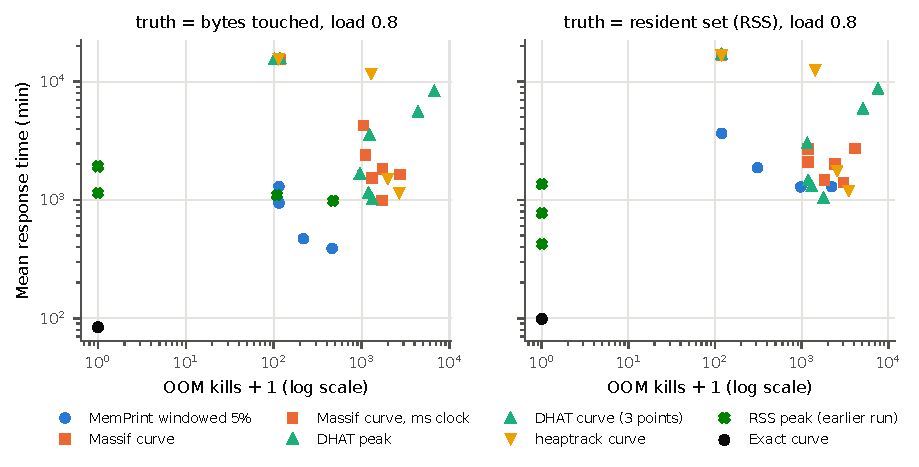
\includegraphics[width=\textwidth]{figures/margin_tradeoff.pdf}
\caption{Mean response time against OOM kills at load 0.8, one marker per margin policy (10\%, 30\%, calibrated
90\% and 100\%). No margin gives a measured estimator both few kills and a short response time, except the
\memprint{} curves under the bytes-touched truth.}
\label{fig:margins}
\end{figure}

\subsection{Margins}

No margin policy rescues an estimator that is badly wrong for some programs (\figref{fig:margins}). A small
margin lets those programs' jobs be killed, and a margin large enough to cover them over-reserves every other
job. With calibrated 100\% margins, every heap profiler must cover GCC's cc1, whose peak it reads at 0.14 to 0.16, so each
job reserves about 6.5 times its estimate and the response time rises to 15{,}000 to 17{,}000 minutes. Before the
LLM engines joined the corpus, the \memprint{} curves needed at most 7 to 19\% under the bytes-touched truth; their
late view of the mapped weights raises that to 40\% at 5\% watched, 136\% at 1\% and 41 times the estimate for
pages only (llama2.c), so with calibrated 100\% margins they give 1{,}299, 4{,}984 and 9{,}440 minutes. Taking each
oracle at its best margin policy changes the order little (\figref{fig:loadbest} in the appendix): under the
bytes-touched truth, \memprint{} windowed at 5\% gives 389 minutes, \memprint{} pages only 469, Massif 991 (1{,}644
with its millisecond clock), DHAT 1{,}011 and heaptrack and gperftools 1{,}154 and 1{,}158.

\subsection{Footprints predicted from source}

\begin{figure}[t]
\centering
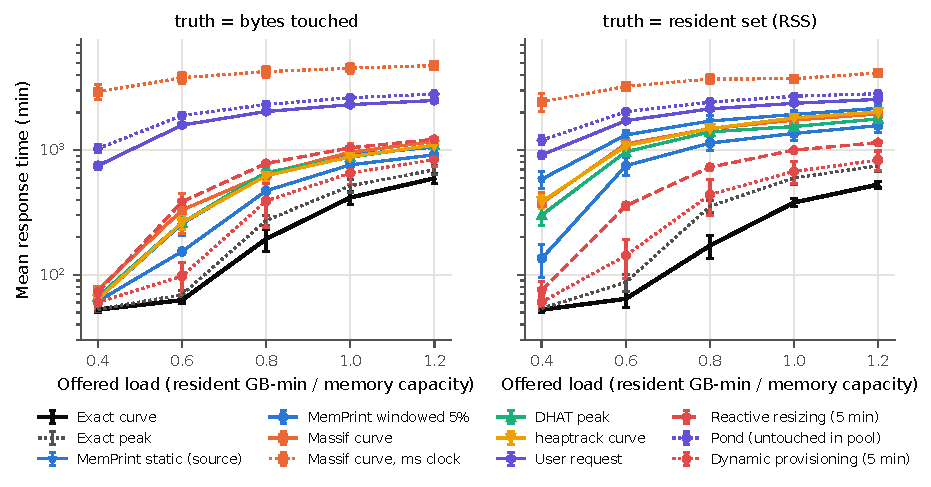
\includegraphics[width=\textwidth]{figures/static_response_vs_load.pdf}
\caption{The nine programs the static route predicts (each at its largest input with a prediction): mean response
time against offered load, calibrated 90\% margins.}
\label{fig:static}
\end{figure}

The static route predicts nine of the programs (PolyBench 2mm, gemm and jacobi-2d at MEDIUM and atax at LARGE,
HPCCG 64, LULESH 30 and NPB IS, CG and MG at class W), and we replay a stream made of those programs alone
(\figref{fig:static}). Their footprints are flatter than those of the full corpus, so the exact peak comes close
to the exact curve (273 against 194 minutes at load 0.8 under the bytes-touched truth). With calibrated 90\%
margins, the static predictions give 642 minutes, against 471 minutes for \memprint{} windowed at 5\%, 623 for
heaptrack, 642 for Massif, 662 for the DHAT peak and 2{,}038 for the request, a 3.2$\times$ gain over the request without running
the program. Two predictions cause most of the static oracle's 343 kills per stream: NPB MG is 7 to 9\% short,
and the margin calibrated on the other eight programs is 0\%, which does not cover it. LULESH is over-predicted by 1.57
times, which wastes memory rather than causing kills. Under the RSS truth the static curve, like the windowed one,
needs more headroom, and it gives 1{,}709 minutes against 1{,}399 for the DHAT peak.

\subsection{LLM inference jobs}
\label{sec:llm}

\begin{figure}[t]
\centering
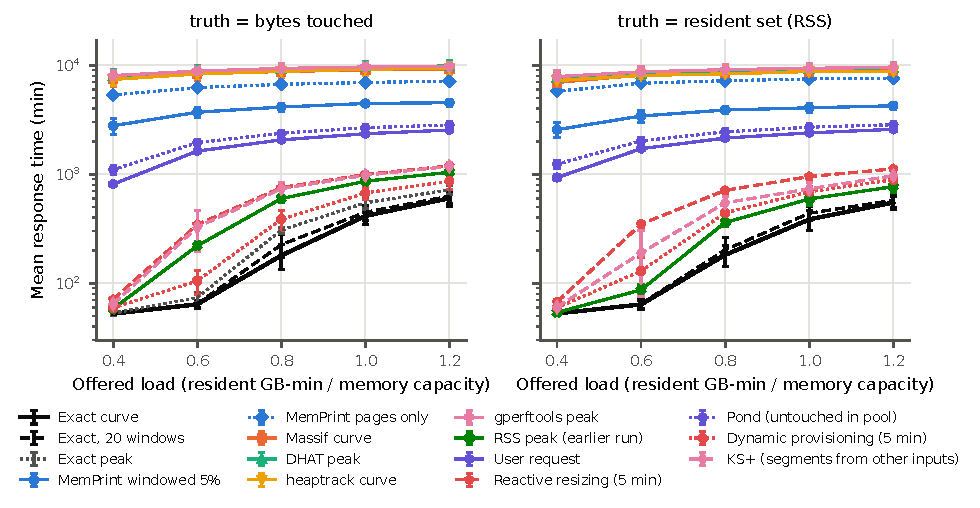
\includegraphics[width=\textwidth]{figures/llm_response_vs_load.pdf}
\caption{A stream of LLM inference jobs alone (llama2.c with three models, llama.cpp with two lengths): mean
response time against offered load, calibrated 90\% margins, each configuration's margin calibrated on the other
four.}
\label{fig:llm}
\end{figure}

\begin{table}[t]
\centering
\caption{The LLM stream at offered load 0.8, calibrated 90\% margins (10\% for the request, ML and reactive
oracles), mean of three seeds; columns as in \tabref{tab:load08}.}
\label{tab:llm}
\resizebox{\textwidth}{!}{\begin{tabular}{lrrrrrrrrrr}
\toprule
 & \multicolumn{5}{c}{Truth = bytes touched} & \multicolumn{5}{c}{Truth = RSS} \\
\cmidrule(lr){2-6} \cmidrule(lr){7-11}
Oracle & Resp. (min) & BSLD & Kills & Res. \% & Used \% & Resp. (min) & BSLD & Kills & Res. \% & Used \% \\
\midrule
Exact curve & 180 & 6.6 & 0 & 76 & 76 & 182 & 6.7 & 0 & 74 & 74 \\
Exact, 20 windows & 226 & 8.6 & 0 & 75 & 72 & 202 & 7.5 & 0 & 76 & 73 \\
Exact peak & 307 & 12.1 & 0 & 75 & 69 & 361 & 14.4 & 0 & 76 & 66 \\
RSS peak (earlier run) & 598 & 24.9 & 0 & 69 & 57 & 361 & 14.4 & 0 & 76 & 66 \\
Reactive resizing (5 min) & 753 & 31.9 & 10 & 65 & 54 & 712 & 29.9 & 9 & 66 & 54 \\
MemPrint windowed 5\%, peak & 785 & 32.9 & 602 & 68 & 51 & 913 & 38.4 & 602 & 68 & 46 \\
ML peak (quantile GBM) & 1836 & 79.1 & 115 & 61 & 36 & 1904 & 82.1 & 115 & 61 & 34 \\
User request & 2067 & 89.3 & 0 & 58 & 33 & 2146 & 92.7 & 0 & 57 & 31 \\
Massif pages-as-heap & 2650 & 114.7 & 0 & 47 & 26 & 2186 & 94.5 & 0 & 52 & 30 \\
Massif pages-as-heap, ms clock & 2955 & 127.9 & 0 & 45 & 24 & 2495 & 107.9 & 0 & 48 & 26 \\
MemPrint windowed 1\% & 3120 & 135.7 & 1049 & 46 & 24 & 3083 & 134.0 & 1046 & 47 & 23 \\
MemPrint windowed 5\% & 4134 & 180.6 & 1034 & 43 & 19 & 3884 & 169.6 & 1033 & 44 & 19 \\
MemPrint pages only & 6685 & 293.2 & 610 & 29 & 9 & 7208 & 316.3 & 1220 & 30 & 9 \\
Massif curve & 8747 & 381.2 & 1195 & 32 & 9 & 8528 & 372.3 & 1195 & 32 & 10 \\
heaptrack curve & 8794 & 383.2 & 1195 & 32 & 9 & 8333 & 363.2 & 1195 & 32 & 10 \\
Massif curve, ms clock & 8869 & 386.7 & 1195 & 32 & 9 & 8630 & 376.5 & 1195 & 32 & 10 \\
DHAT curve (3 points) & 9103 & 397.6 & 1195 & 31 & 9 & 8776 & 383.4 & 1195 & 32 & 9 \\
DHAT peak & 9198 & 400.7 & 1195 & 31 & 9 & 8986 & 391.7 & 1195 & 32 & 9 \\
gperftools peak & 9344 & 408.0 & 1195 & 31 & 9 & 9108 & 397.5 & 1195 & 32 & 9 \\
DHAT hold-then-decay & 9561 & 417.3 & 1195 & 31 & 8 & 9251 & 404.3 & 1195 & 32 & 9 \\
\bottomrule
\end{tabular}
}
\end{table}

To see how the estimators fare on a kind of job whose memory is mostly read-only model weights, we replay a
stream made of the LLM engines alone (\figref{fig:llm}, \tabref{tab:llm}). Each job takes the footprint and the
estimates of one of the five traced configurations (llama2.c with the 15M, 42M and 110M models, and llama.cpp
with 32 and 128 tokens), and each configuration's calibrated margin comes from the other four, as a site that has
run other models or lengths of the same engines would set it.

These footprints are flat, so the curve gains less over the peak than in the full corpus: at load 0.8 the exact
curve gives 180 minutes, the exact peak 307 and the request 2{,}067 under the bytes-touched truth, a 1.7$\times$
gain of the curve over the peak against 5.3$\times$ for the full corpus. The best measured estimate is the RSS
peak of an earlier run, 598 minutes with no kills under the bytes-touched truth and equal to the exact peak under
the RSS truth, because the weights the RSS counts are the footprint. Reactive resizing gives 753 minutes and
\memprint{}'s 5\% peak 785 minutes, 602 kills per stream.

Every heap profiler fails. They read llama2.c at 0.08 to 0.21 of its peak and llama.cpp at about 1.05, so the
margin calibrated on the other configurations cannot cover llama2.c's jobs, which would need headroom of 3.8 to
10.6 times the estimate: with calibrated margins Massif, DHAT, heaptrack and gperftools give 8{,}747 to 9{,}344 minutes and 1{,}195
kills per stream, four times the request. With a fixed 10\% margin, llama2.c's jobs are killed until the requeue
factor has raised their reservation enough, 9{,}050 to 9{,}647 times per stream for DHAT, Massif and gperftools
(15{,}661 for heaptrack), and their response of 613 to 823 minutes hides that waste. Massif with \texttt{--pages-as-heap} counts the file mapping and never under-reads, so it is never
killed, but it over-reserves (2{,}650 minutes).

\memprint{}'s curves fail for a different reason. Its peaks are about right (0.86 to 1.00 of the true peak at 5\%
watched), but its curves reach the peak late (\secref{sec:corpus}), while every job's footprint jumps to the
weights in the first percent of its run. A curve reservation is therefore too small at the start of every job,
and the configurations need 17 to 96\% headroom at 5\% watched; the calibrated margin covers some and not others,
and the curves give 3{,}120 to 6{,}685 minutes with 610 to 1{,}049 kills per stream. Pages only, which never watches,
needs headroom of 20 to 41 times its estimate for llama2.c. This is the same finding as under the RSS truth, from another
cause: a curve is worth only as much as its timing, and \memprint{}'s windowed timing misses memory that a
program maps and reads before the first window. Tracking the residency of file mappings between windows, as the
windowed mode already does for heap blocks, might address it; we have not tested it.

\subsection{Memory needed for the same service}

\begin{figure}[t]
\centering
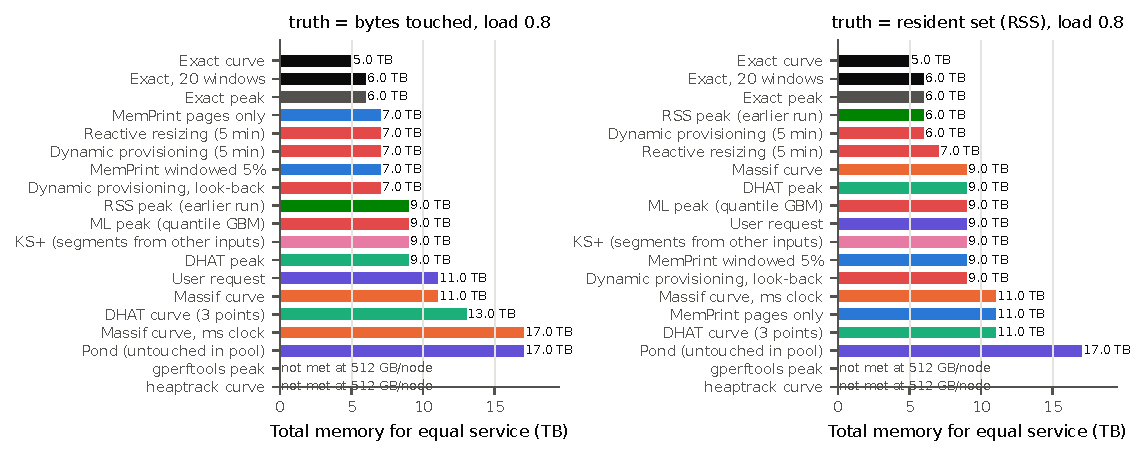
\includegraphics[width=\textwidth]{figures/capacity.pdf}
\caption{The total memory (32 nodes of local DRAM plus the 1\,TB pool) each oracle needs to keep the mean
bounded slowdown within 1.5 times that of the exact curve at 128\,GB per node, at a fixed arrival rate (load 0.8
on the 128\,GB cluster). Local memory per node was swept over 64, 96, 128, 160, 192, 256 and 320\,GB.}
\label{fig:capacity}
\end{figure}

The response-time gains translate into memory a site would have to buy (\figref{fig:capacity}). At a fixed
arrival rate, the exact curve meets the target with 128\,GB per node (5.0\,TB in all). Under the bytes-touched
truth, the exact peak needs 160\,GB per node (6.0\,TB, 20\% more), \memprint{}'s windowed and pages-only curves
and reactive resizing 192\,GB (7.0\,TB, 40\% more), DHAT, an earlier run's RSS and the ML peak 256\,GB (9.0\,TB,
80\% more), and Massif's curve and the request 320\,GB (11.0\,TB, 120\% more). gperftools, heaptrack, Massif's
curve on its millisecond clock and the DHAT curve do not meet the target even at 320\,GB per node. With the LLM
engines in the corpus, \memprint{}'s curves need one step more than before (192 instead of 160\,GB per node), and
gperftools and heaptrack fall from 256\,GB to never, through their calibrated margins. Under the RSS truth, the
exact peak and the RSS of an earlier run need 6.0\,TB, reactive resizing 7.0\,TB, \memprint{} windowed at 5\%,
DHAT, Massif, the ML peak and the request 9.0\,TB, and \memprint{} pages only 11.0\,TB, which repeats the finding
that a curve on a reference clock loses its advantage against a wall-clock truth.

\subsection{What each estimator's cost buys}

\begin{figure}[t]
\centering
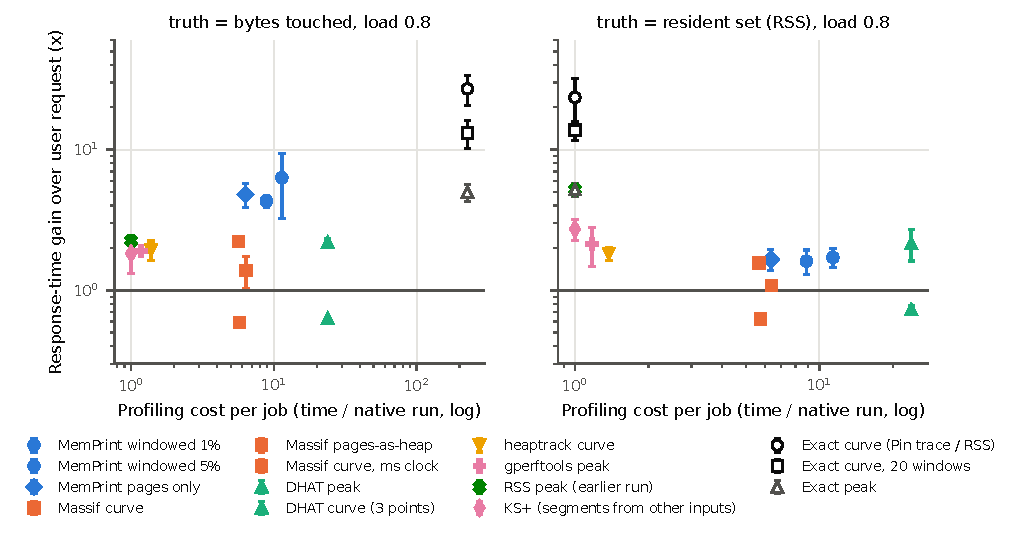
\includegraphics[width=\textwidth]{figures/roi.pdf}
\caption{Profiling cost per job (median time over the native run, at the largest inputs) against the gain in
mean response time over the user's request, at load 0.8, each oracle at its best margin policy. The exact
curve's cost is the full Pin trace under the bytes-touched truth and an RSS sampler under the RSS truth.}
\label{fig:roi}
\end{figure}

\figref{fig:roi} sets each estimator's cost against what it buys. Under the bytes-touched truth, the full Pin
trace costs 227 times the native run and gives a 26.4$\times$ gain over the request as a curve, or 4.9$\times$ as a
peak. \memprint{} windowed at 5\% costs 11 times the native run and gives 5.7$\times$, about a fifth of the exact
curve's gain at a twentieth of its cost; pages only and windowed at 1\% cost 6 and 9 times and give 4.7$\times$ and
4.3$\times$. heaptrack and gperftools cost under 1.5$\times$ and give 1.9$\times$, DHAT costs 24$\times$ and gives
2.2$\times$, and Massif's curve costs 5.7$\times$ and gives 2.2$\times$ (1.3$\times$ with its millisecond clock). An
earlier run's RSS costs nothing extra and gives 2.2$\times$ under the bytes-touched truth, and under the RSS truth it
is the truth's peak. Under the RSS truth the measured curves give 1.6 to 1.7$\times$ and the heap profilers' peaks
1.8 to 2.1$\times$, so the profiling cost buys little until the curve's time axis is fixed.


\section{DHAT curves}
\label{sec:dhat}

DHAT records the heap at its global peak (t-gmax), the time of that peak, and the heap at exit, but no time
series~\cite{ValgrindDHAT}. A scheduler can use those three points in two ways besides the peak. The
\term{DHAT curve} rises linearly from zero to the peak at its recorded time and falls linearly to the exit value.
The \term{hold-then-decay} curve holds the peak from the start to its recorded time, which is safe before the
peak, and falls linearly afterwards. Only "never above the peak" is guaranteed by what DHAT records, and that is
the DHAT peak oracle.

\begin{figure}[t]
\centering
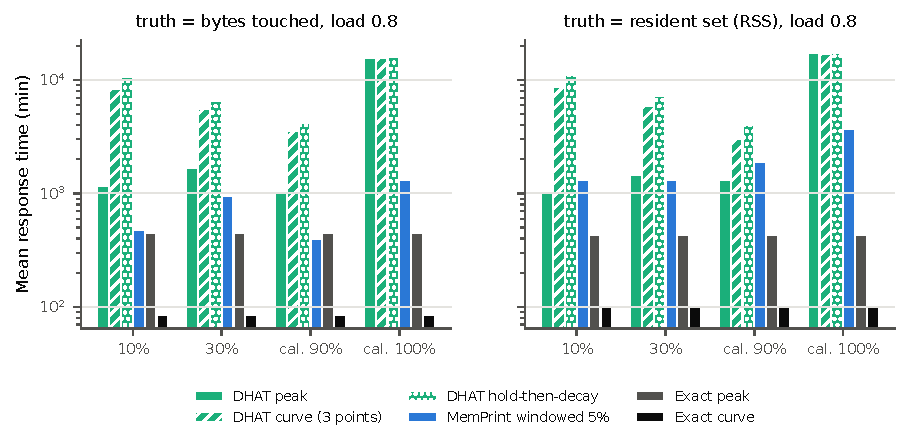
\includegraphics[width=\textwidth]{figures/dhat_curves.pdf}
\caption{DHAT's peak and the two curves built from its three recorded points, against \memprint{} windowed at
5\% and the exact peak and curve, at load 0.8 under each margin policy (log scale).}
\label{fig:dhat}
\end{figure}

Both DHAT curves do worse than the DHAT peak under every margin policy and both truths, except with calibrated
100\% margins, where all three reserve for GCC's cc1 and give about the same (15{,}000 to 17{,}000 minutes;
\figref{fig:dhat}). At load 0.8 with calibrated 90\% margins, the DHAT curve gives 3{,}512 minutes and the
hold-then-decay curve 4{,}161 minutes, against 1{,}011 minutes for the DHAT peak, under the bytes-touched truth, and
3{,}008, 3{,}943 and 1{,}302 minutes under the RSS truth. With fixed margins the curves are worse still (8{,}263 and
10{,}648 minutes at 10\%), because they fall below the truth wherever a program has more than one phase, and their
jobs are killed 5{,}751 to 7{,}642 times per stream. The median program needs 36\% headroom on the DHAT curve (21\%
on hold-then-decay) and the 90th percentile needs 90\% (\tabref{tab:margins}). The average of the DHAT curve over
the run is 0.81 times the true mean footprint at the median over the 71 (program, input) pairs, so it
under-reserves on average as well as in places. DHAT's three
points therefore do not substitute for a measured curve. The information that makes a curve useful to a
scheduler is the timing of every phase, and DHAT records the timing of one.


\section{Limitations}
\label{sec:limits}

The results rest on a model of a cluster and of its jobs, and each simplification limits what they show.

\paragraph{Scaled footprints.} The corpus programs peak at 15 to 450\,MB, and the simulated jobs at tens to
hundreds of GB. Scaling a measured curve to a job's size keeps its shape and every estimator's ratio to the
truth, but it assumes the ratio does not change with the input. The corpus shows that it often does at small
inputs: \memprint{} windowed at 5\% reads 0.61 to 0.92 times the peak of the PolyBench kernels at SMALL, and 1.00
at LARGE. We use the largest input of every program to keep this effect small.

\paragraph{Time axes.} Every curve is put on the job's progress by linear rescaling of its own clock. The true
footprint of a job over wall-clock time is known only for the RSS truth, so the bytes-touched truth favours the
\memprint{} curves, which share its clock of memory references (\secref{sec:results}).

\paragraph{The job stream.} The main stream is synthetic, with memory the contended resource by design, and the
used-to-requested ratio comes from the LANL CM5 log of 1994 to 1996, the only archive log with both fields that we
found. A real trace with requested and used memory per job would test whether the effect holds at the
memory pressure of a production system.

\paragraph{Scheduler and machine.} Jobs use one node, the slowdown is linear in the remote share of the
footprint with one $\beta$ for every job, the pool has no bandwidth contention, and only FCFS with EASY
backfilling was tested. The OOM model requeues a killed job with 1.5 times its reservation, and a batch system
that killed a job only once, or that swapped instead of killing, would change the kill counts.

\paragraph{Costs.} The costs were measured with up to 15 runs sharing the node, so they are slowdowns under
load, and Pin's fixed start-up cost weighs heavily on runs of a few seconds. Longer jobs would amortise it.

\paragraph{LLM inference.} The LLM jobs are single completions of 32 to 128 tokens on the CPU, scaled like every
other program. A serving engine that runs for hours fills its KV cache over many requests, and a GPU engine keeps
its weights in device memory, so neither shape is covered here. llama.cpp's 360M model could not be traced, so the
corpus has llama.cpp at two inputs of one model.

\paragraph{The static route.} The static predictions cover 9 of the 25 programs. They predict a whole-run
footprint for C++ programs, so a program that frees and reallocates its data, such as LULESH, is over-predicted,
and the interpreter takes up to 5.5 hours for one input of NPB CG.


\section{Conclusion}
\label{sec:conclusion}

An exact footprint is worth most to a scheduler on disaggregated memory as a curve over the job's run, and
the gain comes from letting jobs with peaks at different times share memory. On our corpus and streams, the
exact curve gives a 26.4$\times$ shorter mean response time than the user's request and needs 5.0\,TB where the
request needs 11.0\,TB. Heap profilers get most peaks right, but their large errors on a few programs, which
come from memory that is mapped outside the heap or allocated and never touched, cannot be covered by any margin
without over-reserving every other job; LLM engines, whose weights are a file mapping, add a third such program,
which pushes the calibrated margins of heaptrack and gperftools past twice their estimates. Among measured
estimators, \memprint{} windowed at 5\% comes closest to the exact curve, with the smallest margin (6\% for 90\% of
programs) and 40\% more memory than the exact curve for the same service, at 11 times the native run time. On LLM
jobs alone it fails, because its curve learns of the weights only in its windows, while the footprint reaches its
peak in the first percent of the run; there an earlier run's RSS peak is the best measured estimate. DHAT's three recorded points do not make a
usable curve. Two results set the direction of further work. First, under the RSS truth every measured curve
loses its advantage because its clock is not wall-clock time, so \memprint{} should record the native time of
each snapshot and estimate resident pages as well as bytes touched. Second, the static route predicts footprints
without running the program, but its errors on programs that free and reallocate memory, and its cost on large
inputs, limit it today to programs whose footprint is set by their input sizes.

\appendix
\section{Additional figures}

\begin{figure}[h]
\centering
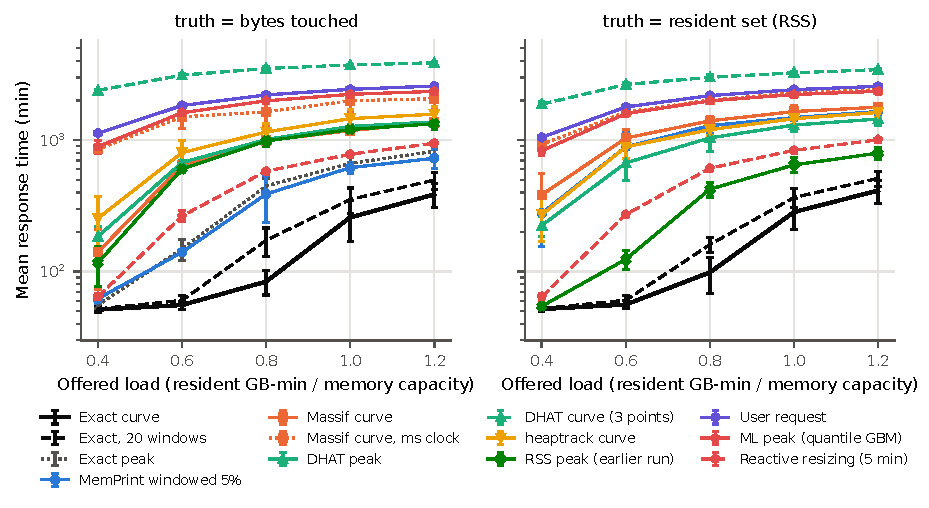
\includegraphics[width=\textwidth]{figures/response_vs_load_best.pdf}
\caption{Mean response time against offered load, each oracle at its best margin policy at each load.}
\label{fig:loadbest}
\end{figure}

\begin{figure}[h]
\centering
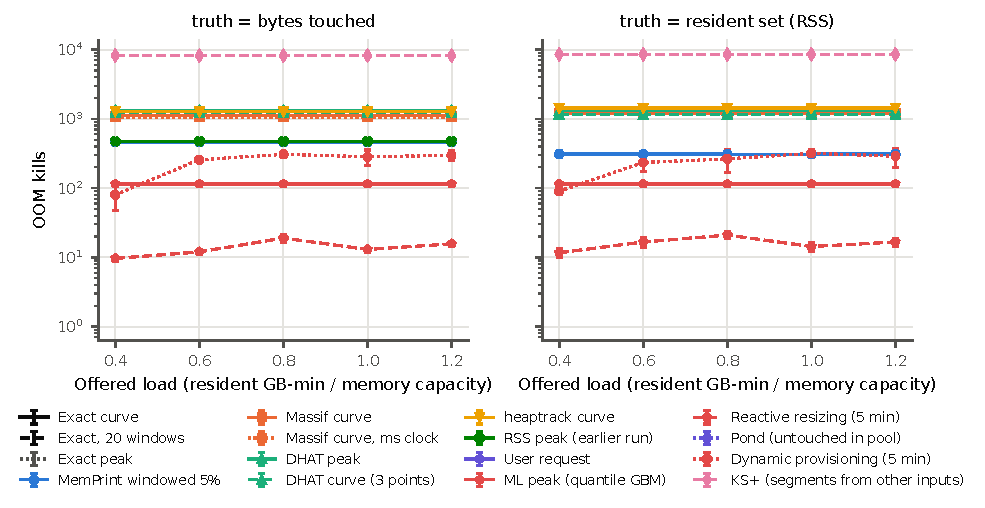
\includegraphics[width=\textwidth]{figures/kills_vs_load.pdf}
\caption{OOM kills per stream of 3{,}000 jobs against offered load, calibrated 90\% margins.}
\label{fig:kills}
\end{figure}

\bibliographystyle{plain}
\bibliography{references}

\end{document}
